\chapter[Project Management]{Project Management}
\label{ch:management}

\chapterepigraph{``All things are created twice; first mentally; then physically.  The key to creativity is to begin with the end in mind, with a vision and a blue print of the desired result."}{ Stephen Covey}

\begin{fullwidth}

\newthought{Project management} is often incorrectly considered to be the coordination of steps a project must move through to be completed on time, the real challenge of project management is constantly incorporating the requirements of the customer into an ever changing system to ensure that the progression of the project is always in the customers interest. A major concern of project management is to minimise wasted time and resources without compromising the quality of the project, wasting time on this project would result in a poorer quality product.

\section{Roles and Responsibilities}
\label{section:roles}

\begin{description}
    \item[Project Manager] Responsible for overseeing the project in general, including managing a schedule, organising meetings and collaborative development sessions. Makes decisions involving tradeoffs between project time, cost, and quality. 
     
    \item[Customer Liaison] Meets with the customer at regular intervals to discuss the project progress, outlook, and any issues which are require customer input.
     
    \item[User Manager] Finds end users to test the product in the later stages of development, then provides feedback to the project manager and team leader. Prime responsibility is to identify issues which are not clearly visible from the project development perspective, but are more apparent to end users.
     
    \item[Analyst] Responsible for ensuring the customer requirements are addressed during planning and development stages of the project, and ensures that the solution will sufficiently address the customers needs.
     
    \item[Graphic Designer] Responsible for prototyping and developing graphical design elements, such as ship sprites, terrain, maps and user interface.
     
    \item[Software Librarian] Ensures team completes documentation to a sufficient standard for long term maintenance. 
     
    \item[Line Manager] Oversees day to day development, intervenes if a developer is off track, ensuring minimal time is wasted perusing low priority work.
     
    \item[Code Reviewer] Responsible for interpreting other developer's code, checking for logical inconsistencies and familiarising themselves with the project as a whole.
     
    \item[Chairman] Responsible for coordinating meetings, ensuring all issues are resolved or at the least discussed, and that all meeting participants have a chance to voice concerns and contributions.
     
    \item[Testing and Integration Manager] Ensures the code is thoroughly tested for bugs, and discovered bugs are flagged and dealt with in reasonable time. Responsible for managing integration testing to prevent bugs occurring on the master branch.
     
    \item[Security Officer] Checks for security flaws in the product, performs security evaluations (such as penetration testing) to ensure the product is sufficiently secure.
     
    \item[Team Leader] Responsible for coordinating the project team, ensuring team members are working to the best of their ability, responsible for making decisions when the there is no clear solution to a particular problem.
      
    \item[Lead Developer] Consults other developers when there is development difficulty, similar responsibilities to Team Leader but makes decisions primarily about the software development itself,  also responsible for enforcing programming style and technique.
     
    \item[Music Composer] Composes soundtrack for the game, must produce a product which the team leader is satisfied with.
    
    \item[Tester] Performs general code testing (e.g. unit tests, component tests).
    
    \item[Programmer] Performs the day-to-day programming specified by the line manager.
    
    \item[Gameplay Design] Critically analysis gameplay design and experience, giving feedback to the team leader on how to improve the games's appeal.
\end{description}

\begin{table*}
	\begin{tabular}{l p{38em}}
		\toprule
		\emph{Person} & \emph{Description} \\
		\midrule
		\emph{Laith Alissa} & Project manager, Customer Liaison, User Manager, Analyst, Graphics Design.\\[0.5em]
		\emph{Jon Cave} & Code Reviewer, Chairman, Security Officer, Testing and Integration.\\[0.5em]
		\emph{Joseph Siddall} & Software Librarian, Line Manager, Testing and Integration.\\[0.5em]
		\emph{Vic Smith} & Team Leader, Lead Developer, Music Composer.\\[0.5em]
		\bottomrule
		\caption{Roles of project group members}
	\end{tabular}
	\label{tab:roles}
\end{table*}
\section{Stakeholders and Communication Plan}
\label{section:communication}

The various parties identified as stakeholders are shown in table \ref{tab:stakeholders} below. The relationship between the stakeholder and the project is shown, along with a rough estimate of their power and interest.\sidenote[][-2em]{See \bibentry{mendelow1991stakeholder}} This grid will form a reference for making sure that all interested parties are communicated with appropriately throughout the duration of the project.

\vspace{1em}

\begin{table*}
	\small
	\renewcommand{\arraystretch}{1.6}
	\begin{tabular}{p{9em} p{5em} p{2.5em} p{2.5em} p{9em} p{9em} p{8em}}
		\toprule
		\emph{Stakeholder} & \emph{Relationship} & \emph{Power} & \emph{Interest} & \emph{Requirements} & \emph{Measurements} & \emph{Communication Strategy} \\
		\midrule
		
		Project Team & Internal & High & High & 
		Good working environment, creative input. & 
		Meeting project spec, good grades! & 
		Various, detailed elsewhere. \\
		
		Supervisor --- Sara Kalvala & Internal & High & High & 
		requirement & 
		Adherence to spec, good PM, high quality write-up. & 
		Weekly meetings. \\
		
		Client --- Matt Leeke & Core \mbox{External} & High & High & 
		requirement & 
		measurement & 
		Weekly meetings. \\
		
		Second Assessor & Core \mbox{External} & High & Low & 
		requirement & 
		measurement & 
		Deliverables only. \\
		
		Projects Organiser --- Steve Matthews & External & High & Low & 
		requirement & 
		measurement & 
		Email or meeting if required. \\
		
		Playtesters & External & Low & High & 
		requirement & 
		measurement & 
		Email. \\
		
		Other future users & Rest of World & Low & High & 
		requirement & 
		measurement & 
		Website, forums, blog. \\
		
		The Haskell and FP Communities & Rest of World & Low & High & 
		requirement & 
		measurement & 
		Online as above, and via the final report. \\
		\bottomrule
	\end{tabular}
	\vspace{1.5em}
	\caption{Stakeholders for the project.}
	\label{tab:stakeholders}
\end{table*}

\noindent Communication within the project team is examined in detail elsewhere in this document, so the remainder of this section is concerned with the other stakeholders.

\subsection{Supervisor Meetings}

Regular communication with the project supervisor is likely to be a critical factor in success of the project. For this reason a weekly meeting with at least one member of the group if not more will be high priority.

\subsection{Client Meetings}

The client is clearly vital to the success of the project, and continual feedback on each release will allow for early identification of any problems. At least one meeting per release (ie each week) will be required, as well as further meetings and correspondence as needed.

\subsection{Projects Organiser and Second Assessor}

The projects organiser could exert a strong influence over the project if they wished, but as there are many projects and it would be inappropriate for them to demonstrate partiality, extended levels of communication are unlikely to be necessary. Brief updates pertaining to deliverables is all that should be required. But if the project organiser initiates communication then they should be made a high priority.

Communication with the second accessor is, for the most part, not appropriate, excepting when within the remit of the deliverables, i.e. the report and presentation themselves.

\subsection{Playtesters and End Users}

\subsection{The Haskell and Functional Programming Communities}

The overall end goal of the project is not just a game, but an examination of Haskell and Functional Programming as a game development environment. 



\section{Risk Management}
\label{section:risk}
 
A proactive approach to risk management was taken. This technique was chosen in order
to maximise the probability of avoiding risks instead of having to move into `fire-fighting mode'
if something went wrong.\citepage{pressman2010}{page 745}
 
As part of this proactive risk management strategy, a number of potential risks were identified.
These risks are shown in table~\ref{tab:risks} along with their estimated probabilities of occurring
and impact if they were to occur.
 
\begin{table*}
	\small
	\begin{tabular}{l p{\textwidth / 2} l l}
		\toprule
		\emph{Risk} & \emph{Description} & \emph{Probability} & \emph{Impact} \\
		\midrule
		Length underestimate & The time required to develop the software is underestimated & Medium & High \\
		Team member illness & One or more team members unable to work due to illness & Medium & High \\
		Hardware failure & Damage to critical hardware causing loss of data & Medium & Medium \\
		Size underestimate & The size of the deliverable has been underestimated & Medium & Medium \\
		Requirements change & Large number of changes to requirements during development & Low & Medium \\
		Ambiguous requirements & Requirements are not fully understood or misinterpreted leading to
			loss of development time as the specification is recreated & Low & Medium \\
		\bottomrule
	\end{tabular}
	\vspace{1.5em}
	\caption{Risk identification and analysis.}
	\label{tab:risks}
\end{table*}
 
With the risks identified, and their likelihood and consequences estimated it is necessary
to draw up plans to mitigate their effects. There are three types of management strategies 
for individual risks: avoidance strategies to reduce the probability of the risk occurring;
minimisation strategies to reduce the impact of the risk; and contingency plans to deal with
the risk if it does arise.\citepage{sommerville2011}{page 601} It is best to avoid the risk,
but if this is not possible then minimisation of the effects and, finally, contingency plans
should reduce the overall impact of a risk on the project. The mitigation and management
strategies for each risk previously identified are listed in table~\ref{tab:rmm}.
 
\begin{table*}
	\small
	\begin{tabular}{l p{37em}}
		\toprule
		\emph{Risk} & \emph{Mitigation / Management} \\
		\midrule
		Length underestimate & Detailed work breakdown with weekly releases to ensure that
			schedule slippage can be caught early \\
		Team member illness & Well documented code (enforced by the software librarian) so
			that other members can quickly start work on less familiar sections of
			the codebase \\
		Hardware failure & Backups and distributed source control, see section~\ref{section:tools} \\
		Size underestimate & Detailed work breakdown structure \\
		Requirements change & Thorough change management system, see section~\ref{section:control} \\
		Ambiguous requirements & Thorough planning phase \\
		\bottomrule
	\end{tabular}
	\vspace{1.5em}
	\caption{Risk mitigation and management.}
	\label{tab:rmm}
\end{table*}
 
The final stage of the risk management process is monitoring. Throughout the duration of
the project each identified risk was reassessed for changes to its probability and
impact. This allowed the mitigation and management strategies to be revisited to ensure that
they were as effective as possible.
 
The two previously identified risks that actually occurred were team member illness and length underestimate.
On a couple of occasions a team member was ill and unable to attend group work sessions or work to their full
capacity. Fortunately, the team was able to reduce the impact of this by ensuring that the work each individual
was performing was not hindered by an absence. This was done by allocating work tasks to be as separate as
possible to allow more parallel development to occur. Also, an illness was never so severe as to stop a team
member from working for longer than a day or two. However, the issue of length underestimation was more serious.
 
% Length underestimation
%
% 1. More time required for network and GUI than hoped
% 2. (1) slowed the development of the ideal game
% 3. (1) was very informative for our goal of investigation of Haskell for game development
 
The proactive approach to risk management was a good choice. By reviewing the potential
risks before starting the development phase of the project it was much easier to avoid risks that could
have had disastrous consequences for the project. For example, by implementing a thorough backup strategy
prior to any data loss actually taking place it was ensured that no work would have been lost if a hardware
failure had occurred. Continuously monitoring and reassessing these risks was also helpful in preventing
any risks becoming more probable or having a greater impact.

\section{Grievance Policy}
It's imperative to document a grievance guideline to ensure that any grievance procedures are fair and impartial. %ref gov
 Because the developer team is small, an internal dispute would have a high cost to the project, so grievance issues need to be dealt with promptly. 
  
\begin{enumerate}[i)]
    \item{Attempt to resolve the grievance issue informally by the team manager.}
    \item{If the issue cannot be resolved informally, and affects the entire project group, then address the issue at the next meeting and attempt to find a resolution in a group environment.}
    \item{If the issue cannot be solved by a formal group meeting then a managerial confrontation is required to reduce the impact on the project.}
    \item{If the issue still cannot be resolved then a complaint should be made to the module supervisor and university procedure should be followed from then on.}
\end{enumerate}

\section{Agile Methodology and Weekly Releases}

\begin{fullwidth}

The project team has adopted the agile development methodology, the project is broken down into smaller increments which require minimal planning and are unlikely to require long term consideration. Development iterations allow the team to regularly deliver working software, reducing the likelihood of delays going unnoticed and becoming obstructions at a later stage. The development cycle the team has selected requires a component release every Tuesday evening, making each iteration span exactly one week. Each release should include the latest completed iteration of the project, the first milestone will be the game prototype which is scheduled for release on 27th November 2012, further milestones include: beta, and finally the release candidate by 19th March 2013.
%%
%% 19th = Tuesday AFTER term ends- feel free to change that if it's too ambitious :P
%% term dates 
%% http://www2.warwick.ac.uk/study/termdates/
%%
The team has readily adopted pair programming, as well as test-driven development and continuous integration to help maintain code stability through multiple iterations, techniques which are strong advocates of the agile development methodology.

There are aspects to development cycles beyond the milestones and time scheduling, programmer welfare is a large focus of agile development strategies. Ensuring programmers are not overworked or lose interest in the project is an emergent factor in maintaining quality in software projects, and although the team and project managers cannot realistically limit the hours a team member spends programming over a week (mainly due to other programming assignments in parallel to the project), Wednesday afternoons and weekends have been avoided in the weekly timetable to guarantee personal time every week.

\subsection{Standup Meetings}
Standup meetings are held every week to discuss individual progress on the project, any issues an individual has been encountered, and what they will attempt to accomplish in the following week.

\section{Change Management}
As the project develops new ideas and approaches may become apparent, care must be taken to avoid blindly integrating changes into the original specification to protect the project from scope creep. The change management procedure involves assessing the viability and benefits of the change request, deciding whether the change would stop the project meeting the requirements, and if so, whether the customer and managers can reach an agreement which incorporates this change into the project or whether the change request should be rejected. The official protocol has been summarised (overleaf) in figure \ref{change_management_diagram}. Change viability is decided on the difference in cost and time required, whereas the requirements assessment is heavily dependant on the customer, and whether they think such a change would prevent the project meeting their requirements.

\end{fullwidth}
\clearpage

\begin{figure*}[h!]
	\label{change_management_diagram}
	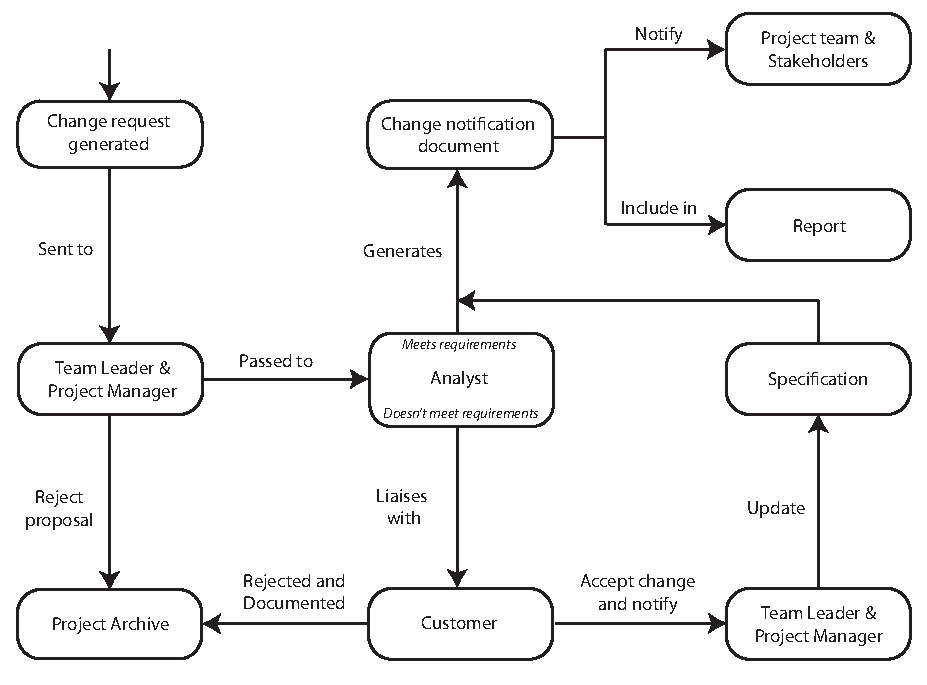
\includegraphics{res/change_management_diagram}
	\caption{Change management workflow}
\end{figure*}

\section{Tools and Techniques}

These are the tools to be used in the day to day running of the project.

\subsection{Source Control: Git}

Source control systems are an essential tool for software projects, especially those
with multiple developers. Using source control to easily track the changes to source
code is helpful because, as McConnell explains, having a history of changes helps a
developer to identify the origin of bugs quickly.\citepage{mcconnell2004}{page 667}

The Git source control system\sidenote{\url{http://git-scm.com/}} has been chosen for this project.
Git was chosen for a number of reasons. Firstly, it has a lightweight branching model which
allows for quick creation of new development branches for experimental features independent of
any other development. Chacon notes this as Git's ``killer feature".\citepage{chacon2009}{page 38}
Another reason for choosing Git is its distributed nature. Every user has a full clone of the
entire repository that can act as a replacement for any other instance of the repository; this means
that there is no single, centralised point of failure.

A centralised master repository will be hosted on Github, a popular code host.\sidenote{\url{https://github.com/}} 
This is to make it easier for team members to share their changes. Once a change has been made
it can be `pushed' to the Github repository; other team members can then `pull' it to their local
repositories.

\subsection{Tracking and Managing Releases: Trello}

\begin{marginfigure}
	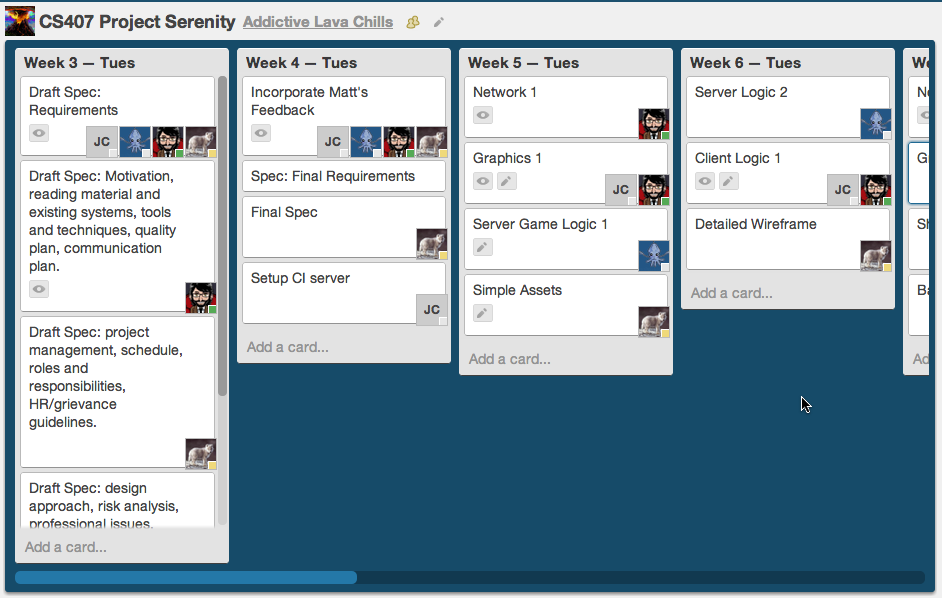
\includegraphics[width=6cm]{res/trello.png}
	\caption{Trello}
	\label{fig:trello}
\end{marginfigure}

Trello is a modern, online take of an age old concept --- a wall of post-its. Trello allows for overall planning of tasks and communication between members in a highly dynamic, fluid way. Cards are arranged into a list-of lists, each list being some kind of functional decomposition or `stovepipe'. Trello has been used in the project to track the requirements for each weeks releases, but still allowing rapid changes to be made and communicated.

\subsection{Bug Tracking: Fogbugz}

Trello does not entirely alleviate the need for a full bug tracker. Fogbugz is a very fully featured service, and has the highly useful feature of automatically converting emails into bugs and auto-assigning them as required.

\subsection{Wiki}
Wiki pages are exceptionally useful for maintaining an informal archive of the project as it develops. The project team uses Github's wiki feature for documenting weekly progress and any issues encountered during agile cycles.

\subsection{Continuous Integration: Jenkins}

Section \ref{section:quality} introduced the idea of continuous integration as a method
of regularly running the test suite and performing a full build of the software.
The Jenkins continuous integration server\sidenote{\url{http://jenkins-ci.org/}}
will be used for this project. Jenkins was chosen because it is a widely used open
source project.\sidenote{\url{http://stats.jenkins-ci.org/jenkins-stats/}}
Jenkins also works well with projects hosted on Github because of its Github plugin\sidenote{\url{https://wiki.jenkins-ci.org/display/JENKINS/GitHub+Plugin}}
and Github's Jenkins specific post-receive hook.

\subsection{Backups}

Backups of the source code and other project assets are essential. In the event of a
disaster, such as losing a computer to a fire, it must be possible to recreate the
entire project in its latest state quickly and without any repetition of work.
The use of Git and Github for source control make it simple to ensure that all
source code is located on multiple computers.
Also, the free service provided by Dropbox\sidenote{\url{https://www.dropbox.com/}}
will be used to share and backup any other files.

\subsection{Cabal}

Cabal is the Haskell package manager and build system. It helps manages dependencies and running of the test suite.

\subsection{Whiteboard}
The project team still finds it extremely useful to brainstorm and refine ideas. Therefore, meetings and programming sessions are routinely scheduled in the vicinity of whiteboards.
